\documentclass[11pt,a4paper]{article}

\usepackage[utf8]{inputenc}
\usepackage[T1]{fontenc}
\usepackage[english]{babel}
\usepackage[margin=2.5cm]{geometry}
\usepackage{graphicx}
\usepackage{booktabs}
\usepackage{tabularx}
\usepackage{xltabular}
\usepackage{float}
\usepackage{listings}
\usepackage{xcolor}
\usepackage{multicol}
\usepackage[hidelinks]{hyperref}

\graphicspath{{figures/}}

% PDDL names in running text (underscores allowed)
\newcommand{\p}[1]{\texttt{\detokenize{#1}}}
\setlength{\emergencystretch}{3em} % long PDDL names do not hyphenate

% PDDL listings for the appendix
\lstset{
  basicstyle=\ttfamily\small,
  columns=fullflexible,
  breaklines=true,
  frame=single,
  commentstyle=\color{gray},
  morecomment=[l]{;},
}

\begin{document}

% ---------------------------------------------------------------------------
% Title page
% ---------------------------------------------------------------------------
\begin{titlepage}
  \centering
  \vspace*{3cm}
  {\Large Planning and Approximate Reasoning (PAR)\par}
  \vspace{0.5cm}
  {\large Final Practical Project\par}
  \vspace{2cm}
  {\huge\bfseries Autonomous Drone Planning for\\[0.3cm] Smart-City Emergency Response\par}
  \vspace{2cm}
  {\Large Sonia Castro Paniello\\[0.2cm] Michelle Miranda\par}
  \vfill
  {\large Master in Artificial Intelligence\par}
  \vspace{0.3cm}
  {\large November 2026\par}
\end{titlepage}

\tableofcontents
\newpage

% Statement, Section 10: 8 to 12 pages, excluding appendices.

\section{Introduction}
% Motivation and scenario summary.

After an emergency in a city, a fleet of autonomous drones has to inspect
damaged locations and bring supplies such as medical kits, water and
communication equipment from depots to the affected locations. Each drone carries one item at a time, and its battery
limits how far it can fly before it needs a charging station. Some areas are
blocked at first and only become reachable once a nearby site has been
inspected or has received its supply. The goal is to
find a sequence of flights, inspections, pick-ups, deliveries and recharges
that meets every demand at the lowest total cost.

In this project we model the scenario in PDDL and solve it with Fast Downward.
Since the planner does not support numeric fluents, the battery is encoded with
symbolic levels. We build two alternative models that differ only in how
recharging works: a full recharge in one action (Model A), or one level per
action (Model B). We test both on a small, a medium and a large instance with
several planner configurations, validate every plan with VAL, and compare
plan quality and search effort.

\section{Problem Analysis}
\label{sec:analysis}
% Search space, types, predicates, actions and design decisions.
We built the model from the problem statement. This section covers what we decided and learned while building it and comparing it with the templates.

\subsection{State and search space}
\label{sec:searchspace}
A state is the set of facts that are true at a given moment. The planner only
matches facts and does not know what a predicate means, so everything the
search needs must be written explicitly. We split the facts into two groups:
\begin{itemize}
  \item \textbf{Static facts}, written once in \p{:init} and never changed:
    the map (\p{connected}, \p{flight_cost}, \p{distance}), the chargers, the
    unlock relations and the battery arithmetic tables.
  \item \textbf{Dynamic facts}, changed by actions: drone position, battery
    level, cargo, supply positions, accessibility, pending inspections and
    pending deliveries.
\end{itemize}
The search space is the set of reachable combinations of dynamic facts. An
approximate \textbf{upper bound} on its size is
\[
  \big(L\,(N{+}1)\big)^{D}\cdot (D{+}2)^{S}\cdot 2^{I},
\]
where $D$ is the number of drones, $L$ the number of locations, $b_0 \ldots
b_N$ the battery levels, $S$ the number of supplies and $I$ the number of
inspection goals. The first term counts, for every drone, its position ($L$
values) and its battery level ($N{+}1$ values). The second term gives each
supply $D{+}2$ possible states: still at its depot, delivered, or carried by
one of the $D$ drones. The last term records whether each inspection has been
done. The exponent $D$ is
why adding drones costs much more than adding locations, which the large
instance shows clearly (Section~\ref{sec:results}).
Table~\ref{tab:grounding} gives the size of the grounded task that Fast
Downward builds for each instance. These numbers are identical in both models.

\begin{table}[h]
  \centering\small
  \begin{tabular}{lrrrr}
    \toprule
    & Small & Medium & Large (1 drone) & Large (3 drones) \\
    \midrule
    Grounded facts   & 23 & 62  & 56  & 103 \\
    Grounded actions & 40 & 316 & 196 & 588 \\
    \bottomrule
  \end{tabular}
  \caption{Size of the grounded task (Fast Downward translator), same in Model A and B.}
  \label{tab:grounding}
\end{table}

\subsection{Types: what never changes}
The base types are \p{drone}, \p{location}, \p{supply} and \p{level}. Supply
kinds are \textbf{subtypes} (\p{medical_kit}, \p{water_package},
\p{communication_device}): the kind of a supply never changes and every supply
has exactly one, so it fits a type. Location roles (charging
station, mission site, locked) are \textbf{predicates} instead: one location
can play several roles at once, and some roles
change during the plan, which a type cannot do. We added no \p{depot}
predicate, following one rule: a predicate is only needed if a precondition or
the goal tests it. No action asks whether a location is a depot. The depot is
simply where the supplies start (\p{supply_at} in \p{:init}).

\subsection{Avoiding negative preconditions}
Several conditions are naturally negative: ``the drone carries nothing'', ``not
inspected yet'', ``not locked'', ``battery not full''. Each one is replaced by
a positive fact that actions add and delete, so the domain only needs STRIPS,
typing, conditional effects and action costs:
\begin{itemize}
  \item \p{cargo_empty}: ``carrying nothing'' written as a negation would also
    need a quantifier over every supply.
  \item \p{needs_inspection}: \p{inspect} requires it and deletes it. A second
    inspection then has no matching fact, and locations nobody asked about
    (depot, charger) cannot be inspected at all, so there are fewer grounded
    actions. \p{inspected} is kept as a separate record because the goal
    checks it.
  \item \p{accessible} instead of \p{locked}: it is true in \p{:init} for every
    location except the locked ones, including every drone start location.
\end{itemize}

\subsection{Locked locations and unlocking}
``Locked'' is not the same as ``needs inspection''. A mission site must be
enterable, otherwise the drone could never reach it to inspect it. A locked
location cannot be entered until one specific event happens: inspecting some
location $X$, or delivering some supply $S$. The problem designer chooses these
pairs, so they are static facts in the problem file:
\p{unlocked_by_inspection(X, Y)} and \p{unlocked_by_delivery(S, Y)}.

\textbf{Delivery is keyed by the supply, not by the location.} If it was only keyed by
location, if a site needed two supplies, the first one would open the door. Adding the location as an extra argument is
redundant: each supply object is needed by exactly one location, so the
supply already fixes where it is delivered.
    
\textbf{Rejected alternative:} blocking the exit of the
unlocking location (a precondition to fly along the lines of "a drone at X can only leave if X is inspected"). It
depends on the map shape, it traps drones
that only pass through $X$, and it cannot express a delivery that unlocks
a location. We kept the check on the \emph{destination},
\p{(accessible ?to)} in \p{fly}.

\subsection{Symbolic battery and plan cost}
Fast Downward has no numeric fluents, so the battery must be symbolic. Our
first idea was one predicate per battery level
(\p{batteryb1(drone)} \ldots \p{batterybn(drone)}), which needs a separate
\p{fly} action for every (start level, cost) pair and changes the domain with
every capacity. Instead, battery levels are objects $b_0 \ldots b_N$ and the
current level is \p{(battery ?d ?l)}, as in the template. One \p{fly} action
then covers every level, and the domain does not depend on the capacity.

We separate \p{connected} (the route exists) from \p{flight_cost} (how many
levels it consumes, as a level object). The plan cost needs a number:
\p{(increase (total-cost) ?c)} is invalid, because \p{b2} is a name and not a
number, and the planner cannot convert one into the other. The same cost is
therefore stored again in the static numeric function \p{distance}. \p{fly}
adds the distance to \p{total-cost} and every other action adds 1. The two
values must match: otherwise the battery drains one amount while the plan cost
counts another, and VAL still accepts the plan. We checked both lists against
the location diagrams, and every edge is written in both directions, because
the planner only matches facts that are declared.

The planner knows nothing about the order of the levels, so subtraction is a
static lookup table \p{battery_after(before, cost, left)}, with rows only where
$\mathit{before} \geq \mathit{cost}$. A flight with too little battery has no
matching row, so it is never applicable. The table also fixes \p{?left}:
without it, \p{?left} would be a free parameter and a drone could gain battery
while flying. Illegal movements are automatically excluded by the absence of a matching fact.

\subsection{Actions and goal}
The five actions are \p{fly}, \p{inspect}, \p{pick-up-supply},
\p{deliver-supply} and \p{recharge}.  \p{deliver-supply} does not put the supply back on
the map at the destination. Otherwise another empty drone could pick it up
again, which is unrealistic (the supply is used up) and adds pointless
branches to the search. The goal contains only the
mission (\p{inspected}, \p{delivered}), not \p{accessible}: unlocking is a
means, not a mission.

% ===========================================================================
\section{PDDL Implementation}
\label{sec:pddl}
% Commented domain files, with an explanation of every predicate and action.

Both domains (\p{domain-A.pddl}, \p{domain-B.pddl}) are fully commented and
listed in Appendix~\ref{app:pddl}. They differ only in \p{recharge}
(Section~\ref{sec:models}). Both are named \p{drone_emergency}, so the same
problem files serve both models without changes.

\paragraph{Requirements.}
\p{:strips} (add and delete effects), \p{:typing}, \p{:conditional-effects}
(the \p{forall}/\p{when} unlocking) and \p{:action-costs} (\p{total-cost},
\p{distance}). We do not need \p{:negative-preconditions}.

\paragraph{Predicates.}
Table~\ref{tab:predicates} lists every predicate and its meaning.

{\small
\begin{xltabular}{\textwidth}{@{}l X c@{}}
  \toprule
  Predicate & Meaning & S/D \\
  \midrule
  \endfirsthead
  \multicolumn{3}{@{}l}{\footnotesize\emph{Table~\ref{tab:predicates} (continued)}}\\
  \toprule
  Predicate & Meaning & S/D \\
  \midrule
  \endhead
  \bottomrule
  \multicolumn{3}{@{}l}{\footnotesize $^{*}$Each drone carries at most one supply at a time.}\\
  \caption{Predicates (S = static, D = dynamic). Functions: \p{total-cost} and static \p{distance ?from ?to-location}.}
  \label{tab:predicates}
  \endlastfoot
    \p{drone_at ?d-drone ?l-location} & drone \p{?d} is at location \p{?l} & D \\
    \p{carrying ?d-drone ?s-supply} & drone \p{?d} carries supply \p{?s} & D \\
    \p{cargo_empty ?d-drone} & \p{?d} carries nothing$^{*}$ & D \\
    \p{connected ?from ?to-location} & direct flight possible (both directions declared) & S \\
    \p{has_charging_station ?l-location} & \p{?l} has a charger & S \\
    \p{accessible ?l-location} & \p{?l} can currently be entered & D \\
    \p{unlocked_by_inspection ?x ?y-location} & inspecting \p{?x} makes \p{?y} accessible & S \\
    \p{unlocked_by_delivery ?s-supply ?y-location} & delivering supply \p{?s} makes \p{?y} accessible & S \\
    \p{needs_inspection ?l-location} & \p{?l} still has to be inspected & D \\
    \p{inspected ?l-location} & \p{?l} has been inspected (goal) & D \\
    \p{needs_supply ?l-location ?s-supply} & \p{?l} is waiting for supply object \p{?s} & D \\
    \p{supply_at ?s-supply ?l-location} & \p{?s} lies at \p{?l} and is not carried & D \\
    \p{delivered ?s-supply ?l-location} & \p{?s} has been delivered to \p{?l} (goal) & D \\
    \p{battery ?d-drone ?b-level} & current battery level of \p{?d} & D \\
    \p{flight_cost ?from ?to-location ?c-level} & the flight costs \p{?c} levels & S \\
    \p{battery_after ?b ?c ?left-level} & $b - c = \mathit{left}$, only listed if $b \geq c$ & S \\
    \p{next_level ?b ?up-level} & $\mathit{up}=b+1$, no row starts at max & S \\
    \p{max_level ?b-level} & full capacity (read by Model A only) & S \\
\end{xltabular}
}

\paragraph{Actions.}
Table~\ref{tab:actions} summarises every action and its meaning.

\begin{table}[!h]
  \centering\small
  \begin{tabular}{@{}p{2.6cm} p{5.3cm} p{5.6cm} l@{}}
    \toprule
    Action & Preconditions & Effects & Cost \\
    \midrule
    \p{fly} & at origin; connected; destination accessible; current battery;
      flight cost; \p{battery_after} row exists &
      move drone; replace battery level by the remaining one & distance \\
    \p{inspect} & drone at \p{?l}; \p{needs_inspection ?l} &
      add \p{inspected}; delete \p{needs_inspection}; unlock every
      \p{?y} with \p{unlocked_by_inspection ?l ?y} & 1 \\
    \p{pick-up-supply} & drone and supply at the same location; \p{cargo_empty} &
      delete \p{supply_at} and \p{cargo_empty}; add \p{carrying} & 1 \\
    \p{deliver-supply} & drone at \p{?l}; \p{carrying ?s}; \p{needs_supply ?l ?s} &
      delete \p{carrying} and \p{needs_supply}; add \p{cargo_empty} and
      \p{delivered}; unlock every \p{?y} with \p{unlocked_by_delivery ?s ?y} & 1 \\
    \p{recharge} & drone at a charger; current level has a \p{next_level} &
      Model A: level $\to$ max. Model B: level $\to$ level $+1$ & 1 \\
    \bottomrule
  \end{tabular}
  \caption{Actions of both domains.}
  \label{tab:actions}
\end{table}

The full commented code of every action is in Appendix~\ref{app:pddl}. Two
points are worth noting. In \p{fly}, each precondition fixes one unknown
parameter: \p{battery} gives the current level from the state,
\p{flight_cost} the cost from the map, and \p{battery_after} the remaining
level from the table. Nobody passes parameter values: the planner keeps only
the combinations for which every precondition is a true fact. Unlocking, in
\p{inspect} and \p{deliver-supply}, is a conditional effect,
\p{(forall (?y - location) (when (unlocked_by_inspection ?l ?y) (accessible ?y)))}:
``for every location $y$, if this event opens $y$, make it accessible''. Here
\p{?y} exists only inside the \p{forall}. It is not an action parameter, and
if no unlock fact matches, nothing extra happens.


% ===========================================================================
\section{Alternative Models}
\label{sec:models}
% Description and structured comparison of Model A and Model B.

The two models differ only in \p{recharge}. In Model A (full recharge) one action sets the battery to
    \p{max_level}, whatever the current level, at cost 1. In Model B (partial recharge) each action raises the battery
    by one level through \p{next_level}, at cost 1.

An optimal planner never keeps an action that only adds cost like recharging at full batery, but it would still be grounded and tried. Model B blocks it for free, because no \p{next_level} row starts at the maximum. In Model A we first used an
extra static predicate \p{isnotmax}. We then noticed that the starting levels
of the \p{next_level} rows are exactly that list, so Model A also requires
\p{(next_level ?current ?higher)}, only as a ``not full'' check. This removes one predicate and lets both domains
share the same problem files. \p{max_level} is simply ignored by Model B. Both
\p{recharge} actions have the same number of groundings, which is why
Table~\ref{tab:grounding} is identical for the two models.

Table~\ref{tab:models} summarises the evidence from the optimal configuration
(A$^*$ with LM-cut), the full results are in Section~\ref{sec:results}. We analize the differences based on 4 criteria:

\begin{table}[h]
  \centering\small
  \begin{tabular}{@{}lcccccc@{}}
    \toprule
    & \multicolumn{2}{c}{Optimal cost} & \multicolumn{2}{c}{Recharges / length}
    & \multicolumn{2}{c}{Expanded states (time)} \\
    Instance & A & B & A & B & A & B \\
    \midrule
    Small            & 10 & 10 & 1 / 10 & 1 / 10  & 16 (0.2 s)   & 16 (0.1 s) \\
    Medium           & 26 & 31 & 1 / 24 & 6 / 29  & 123k (8.0 s) & 336k (14.2 s) \\
    Large (3 drones) & 30 & 31 & 1 / 26 & 1 / 27  & 115k (58 s)  & 243k (123 s) \\
    Large (1 drone)  & 38 & 50 & 4 / 33 & 16 / 45 & 4.5k (0.4 s) & 11.4k (0.8 s) \\
    Large clustered$^\dagger$ & 31 & -- & 1 / 28 & -- & 420k (203 s) & time limit \\
    \bottomrule
  \end{tabular}
  \caption{Model A vs Model B, A$^*$ + LM-cut, 5 min / 4 GB. $^\dagger$Extra
    experiment (three drones starting at the same depot).}
  \label{tab:models}
\end{table}

  \textbf{Expressiveness.} Model B is more realistic as charging takes
    time roughly proportional to the energy restored. It also allows partial charging, so a drone can take just
    enough energy for the rest of its route. \textbf{Planning complexity.} The grounded tasks have the same size,
    so the difference comes from plan depth. In B the optimal plans are longer
    (up to 12 extra actions), and LM-cut expands about 2--3 times more states. We think part of the reason is the delete relaxation behind the heuristics: the starting battery fact is never deleted there. The more recharge actions a plan needs, the more the heuristic underestimates, and B needs many more. 
    
    \textbf{Plan quality and runtime.} The optimal costs differ exactly by
    the extra recharge actions. In the medium instance and the single-drone
    large instance the flights are the same in both models (13 and 17), and B
    adds 5 and 12 recharges. When only one level is missing (small instance) the two
    models coincide. Runtime follows the expanded states, roughly doubling
    in B. \textbf{Trade-offs.} Model A gains shorter plans and faster search, at
    the cost of a less faithful cost model. Recharging is cheap whatever the
    battery level, so the planner has no incentive to save energy. Model B
    gains realism and plan costs that reflect energy use, at the cost of deeper
    search, which becomes the bottleneck when several drones need several
    levels each.


\section{Problem Instances}
\label{sec:instances}
% Each instance with its location diagram (plots/).

Our master is taught on campuses in Barcelona and Tarragona, so we placed the
instances in the two cities we travel between. The small and medium instances
are flood emergencies in Barcelona, and the large one is a chemical emergency
in Tarragona. We checked every problem file against Section~5 of the
statement before running the experiments.

\subsection{Small instance: Barcelona flood}
A storm floods the Barceloneta district and cuts off Parc de la Ciutadella,
used as an evacuation centre. One drone starts full (\p{b4}) at the El Prat
aerodrome, the depot that holds \p{kit1}
(Figure~\ref{fig:small}). The five locations form a line, and every edge
costs 1. The goals are to deliver
\p{kit1} to Hospital de Viladecans, across the Llobregat, and to inspect
Barceloneta and Ciutadella. Ciutadella is locked until Barceloneta has been
inspected.

\begin{figure}[h]
  \centering
  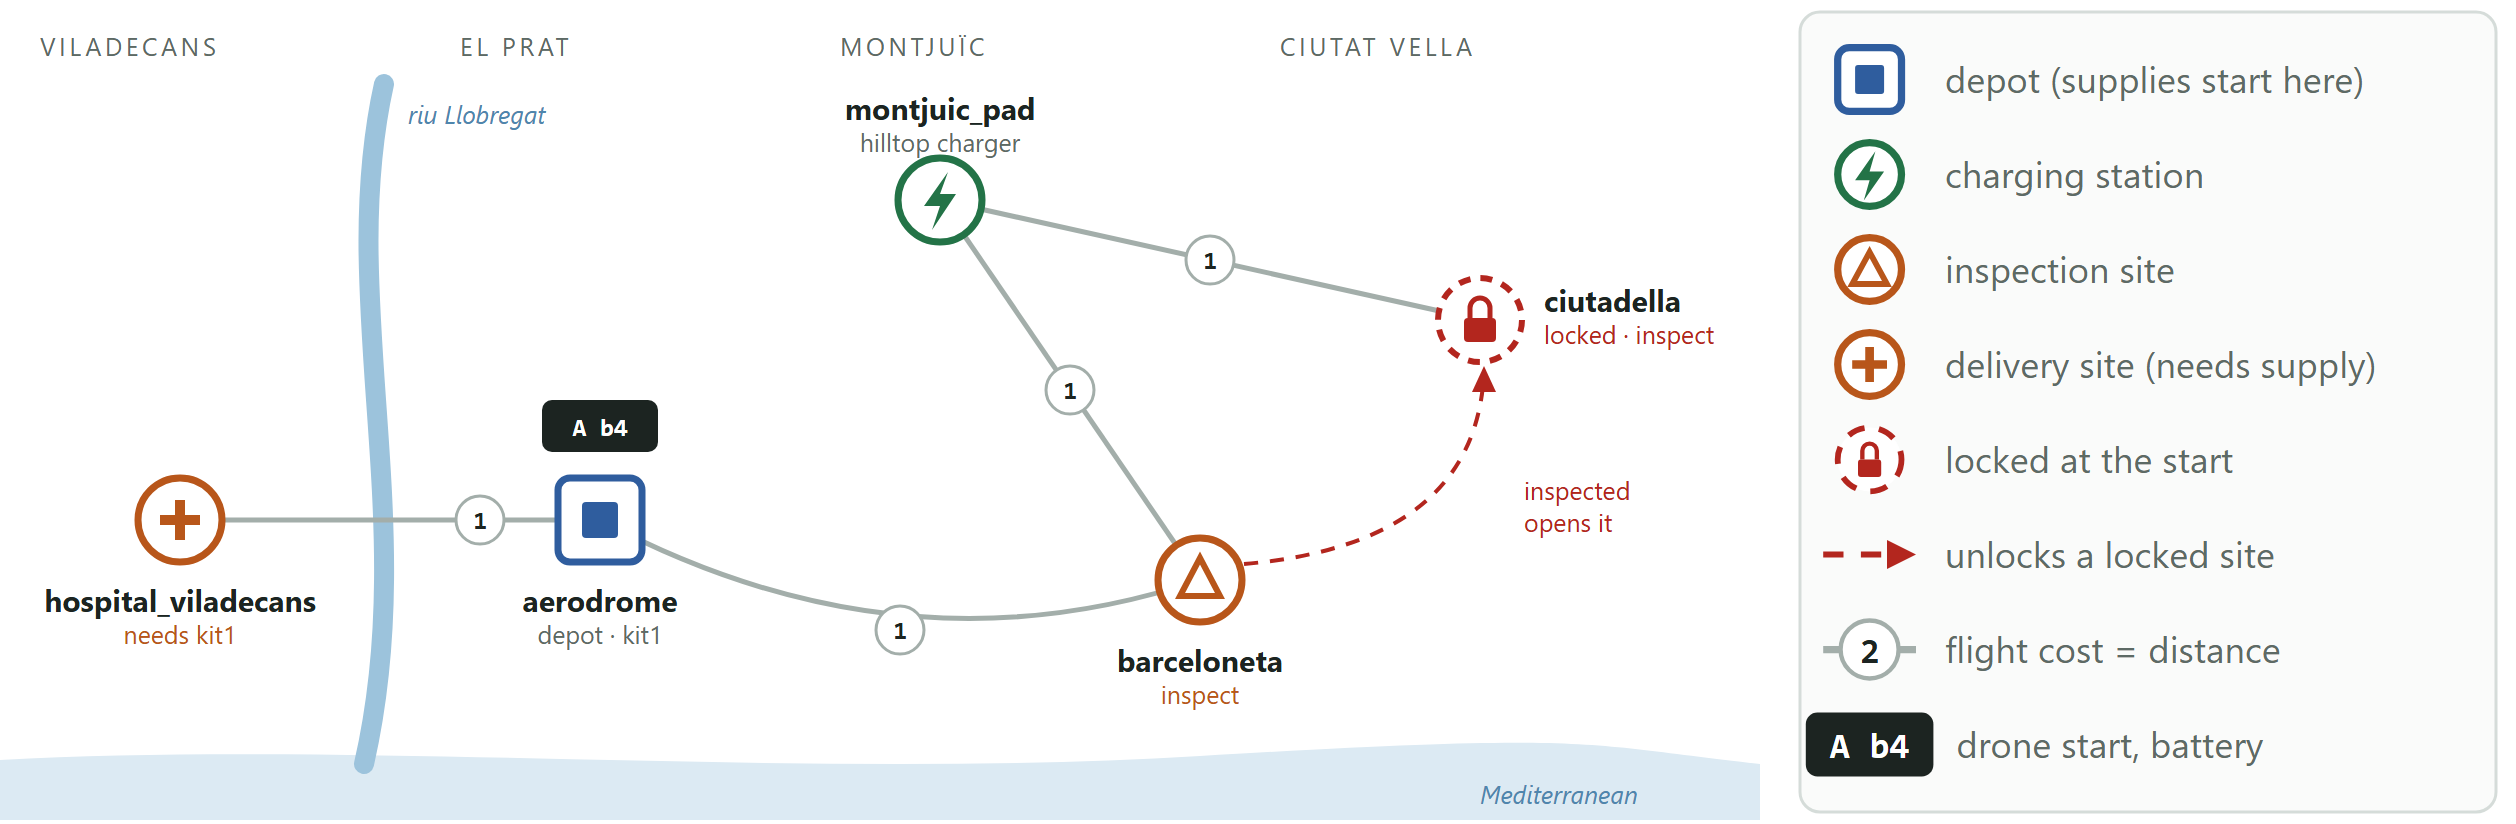
\includegraphics[width=\textwidth]{small-instance.png}
  \caption{Small instance (Barcelona): one drone, five locations, every edge costs 1.}
  \label{fig:small}
\end{figure}

\paragraph{Why a recharge is unavoidable.} The drone starts between the two
ends of the line, and both ends are mission sites. It must reach one end and
come back. The cheapest way is aerodrome $\to$ hospital $\to$ aerodrome and then aerodrome $\to$ barceloneta $\to$ montjuic\_pad $\to$
ciutadella. Every complete mission needs at least 5 flights, which
is 5 levels, more than the 4 of a full battery. A breadth-first search over
the map confirmed that 5 is the minimum. The optimal cost is
10 in both models. In Model B a single \p{b0}$\to$\p{b1} step is enough.


\subsection{Medium instance: Barcelona storm surge}
Flooding hits the coast and the Besòs basin (Figure~\ref{fig:medium}). Two
drones start at \p{port_depot} (\p{b5}) and at the \p{glories_tower} charger
(\p{b4}). There are 8 locations: one depot holding the three supplies, two
chargers and five mission sites. The capacity is \p{b6} and edges cost 1 or
2. The goals are 4 inspections and 3 deliveries of three different kinds
(medical kit, water, communication device).

\begin{figure}[h]
  \centering
  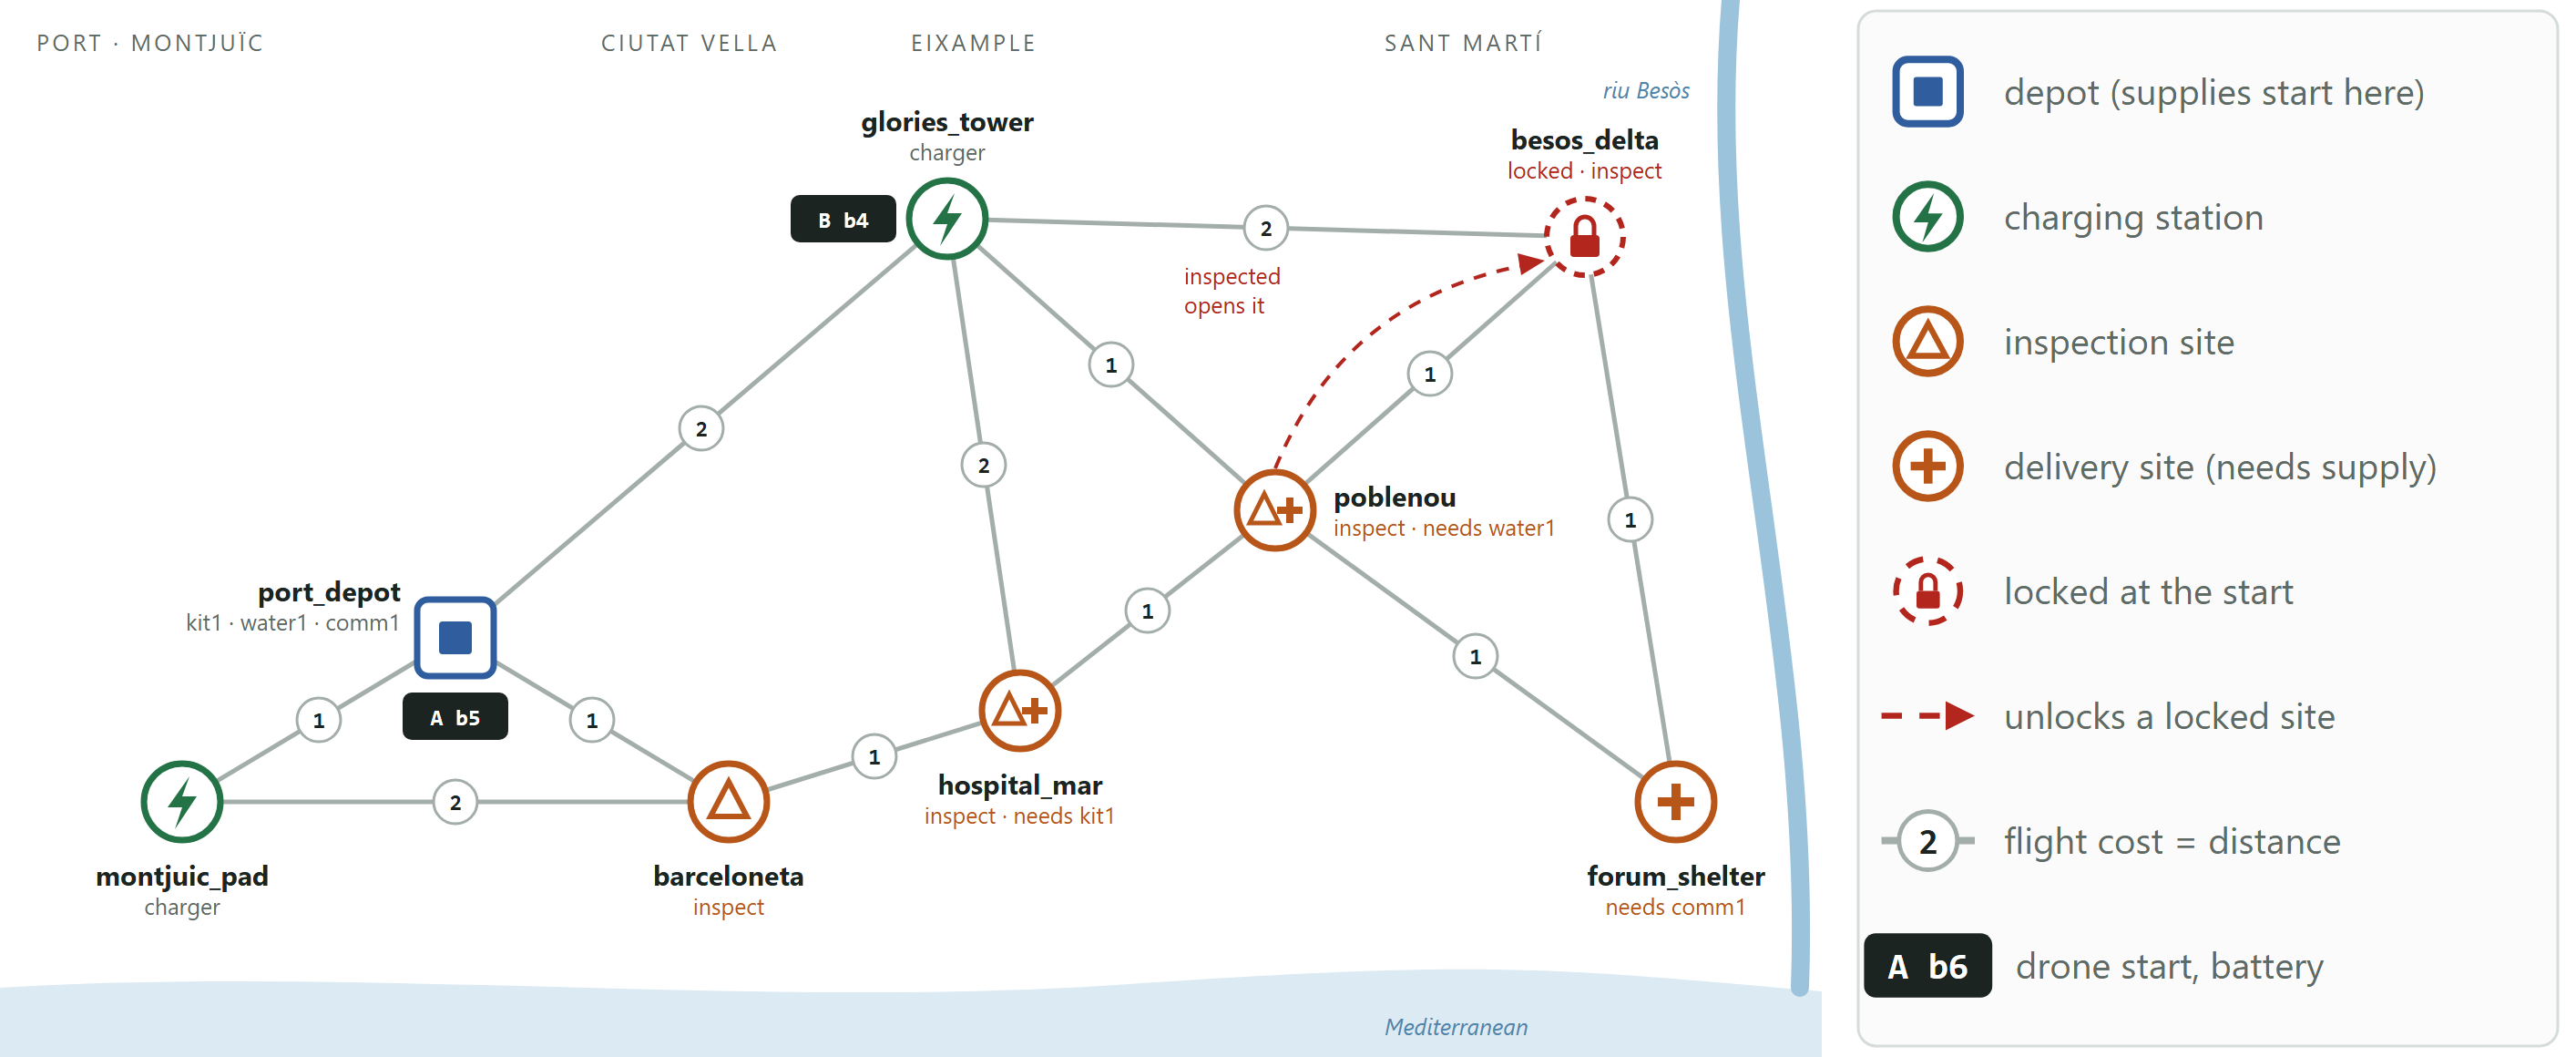
\includegraphics[width=\textwidth]{medium-instance.png}
  \caption{Medium instance (Barcelona): two drones, eight locations, edge costs 1--2.}
  \label{fig:medium}
\end{figure}

\paragraph{The locked site.} \p{besos_delta} is not accessible at the start
and opens when its neighbour \p{poblenou} is inspected. A sequence that fails
is flying there first: \p{(fly droneB glories_tower besos_delta b4 b2 b2)}.
The battery rows and the edge exist, but the precondition
\p{(accessible besos_delta)} of \p{fly} is false, so the action is not
applicable, and every route to the site is blocked the same way. Inspecting \p{poblenou} fires the conditional effect and adds
\p{(accessible besos_delta)}.

\subsection{Large instance: Tarragona chemical leak}
After a leak at the petrochemical park, responders need a radio relay at
Bonavista before drones may enter the park. The old town (Part Alta) stays
closed until the Roman amphitheatre below it has been checked for damage
(Figure~\ref{fig:large}). There are 12 locations: two depots, three chargers
(one of them, \p{bonavista}, is also a delivery site) and mission sites on
both banks of the Francolí. The capacity is
\p{b6} and edges cost 1--3; the longest edge crosses the river. There are 8
goals: 4 deliveries of three kinds and 4 inspections.

\begin{figure}[h]
  \centering
  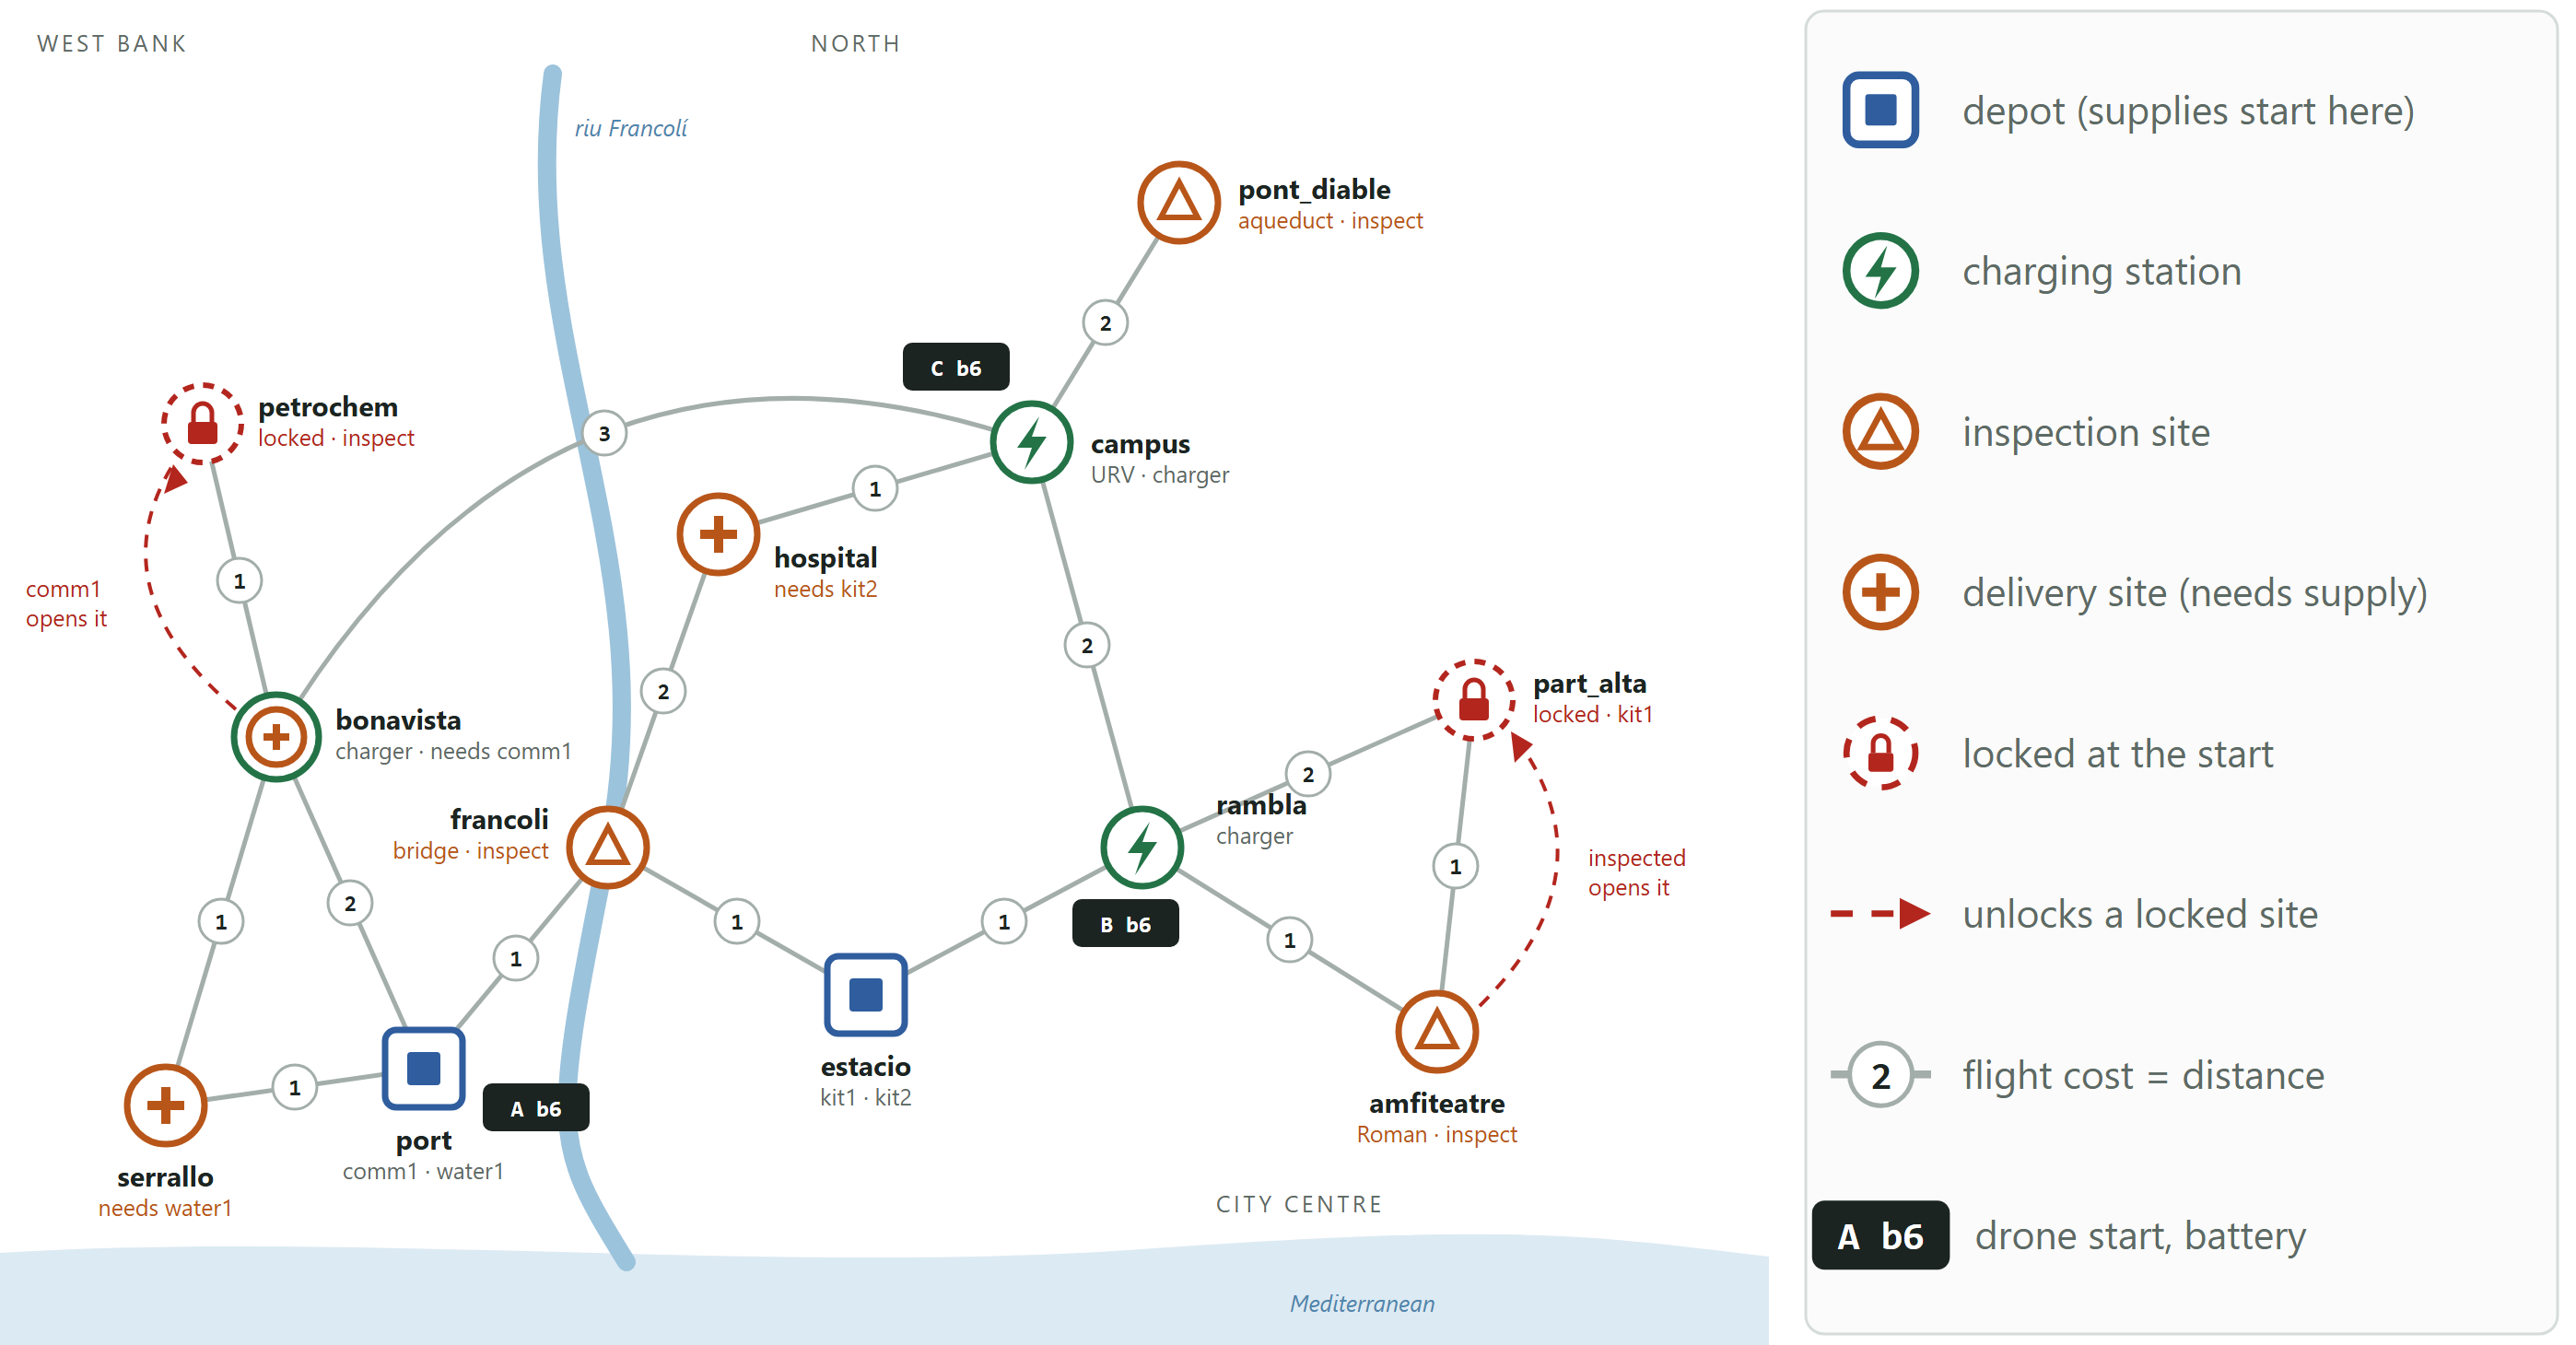
\includegraphics[width=\textwidth]{large-instance.png}
  \caption{Large instance (Tarragona): three drones, twelve locations, edge
    costs 1--3, one delivery lock and one inspection lock.}
  \label{fig:large}
\end{figure}

\paragraph{Locks.} The required delivery lock is
\p{(unlocked_by_delivery comm1 petrochem)}: \p{comm1} must go from the port
to Bonavista, and only then can a drone fly to the park and inspect it. It
works like the inspection lock, but the conditional effect is in
\p{deliver-supply} and the key is the supply. We added an inspection lock as
well: \p{part_alta} opens after \p{amfiteatre} is inspected, so the
\p{kit1} delivery also has an ordering constraint.

\paragraph{Single-drone variant.} Following the hint in the statement, the
three drones start full in different regions: \p{droneA} at the port (west
bank), \p{droneB} at \p{rambla} (city centre) and \p{droneC} at \p{campus}
(north). Each one can serve its own group of sites.
\p{problem-large-1drone.pddl} keeps the same map, goals, supplies and locks
with \p{droneA} only, which must cross the whole city and recharge more often.
Section~\ref{sec:results} compares the costs.

\section{Planner Setup}
\label{sec:setup}
% Tools used, configurations tested, experimental procedure.

\paragraph{Tools.} We built Fast Downward~\cite{helmert2006fd} (commit
\p{487e33c}, October 2026) and VAL~\cite{howey2004val} (commit \p{3c7a1f3})
from source in WSL~2 (Ubuntu 24.04) on Windows
11, on a laptop with an Intel Core Ultra 5 115U and 7\,GB of memory available
to WSL. The exact commands are in \p{README.txt}.

\paragraph{Configurations.} Table~\ref{tab:configs} lists the configurations.
The two required ones are LAMA-first~\cite{richter2010lama} (fast,
satisficing) and A$^*$ with LM-cut~\cite{helmert2009lmcut} (cost-optimal). We added three more so we could see the effect of the
heuristic separately from the effect of the search. A$^*$ with blind, $h^{max}$
and LM-cut keeps the search fixed and uses heuristics that are increasingly
informed (all admissible, so all three return optimal plans).
\p{eager_greedy([ff()])} is a greedy search with plain $h^{FF}$ and no
landmarks or preferred operators, which shows what LAMA-first adds. The
anytime \p{--alias lama} was run on the large variants, as the statement
suggests, because LAMA-first's first plan can be far from the best one.

\begin{table}[h]
  \centering\small
  \begin{tabular}{@{}l p{4.6cm} p{4.4cm} l l@{}}
    \toprule
    Name & Search & Heuristic & Optimal & Instances \\
    \midrule
    lama-first  & lazy greedy, preferred operators & $h^{FF}$ + landmark count (unit costs) & no & all \\
    lama        & lama-first, then weighted A$^*$ ($w$ = 5, 3, 2, 1) & $h^{FF}$ + landmark count & no & large \\
    astar-lmcut & A$^*$ & LM-cut & yes & all \\
    astar-hmax  & A$^*$ & $h^{max}$ & yes & all \\
    astar-blind & A$^*$ & blind & yes & all \\
    gbfs-ff     & eager greedy & $h^{FF}$ & no & all \\
    \bottomrule
  \end{tabular}
  \caption{Fast Downward configurations. Every run: \p{--overall-time-limit 5m --overall-memory-limit 4G}.}
  \label{tab:configs}
\end{table}

\paragraph{Procedure.} One script (\p{run_experiments.sh}) runs every
instance $\times$ model $\times$ configuration with the same limits. It
validates each plan with \p{Validate -v} on the same domain and problem files,
and writes one row per run to \p{results/results.csv}. Plans, VAL outputs and
Fast Downward logs are kept in \p{plans/}, \p{validation/} and \p{logs/}. For
\p{lama}, which writes a cheaper plan file each time it improves, the last
plan is validated and reported. \emph{Runtime} is Fast Downward's ``Planner
time'' (translation plus search), \emph{expanded states} is the last
``Expanded'' value in the log, and \emph{plan cost} is VAL's final value of
\p{total-cost}. An unsolved run is marked as a time or memory failure from the
planner's own message. \p{lama} keeps searching after each plan. It stops early only when its last
weighted A$^*$ iteration ($w = 1$) ends without finding a cheaper plan. Otherwise it runs until the time limit, so
its runtime does not measure how long the best plan took. Its expanded states
count only the last iteration.
All 66 runs were run in one batch on an idle
machine, so the runtimes are comparable. 57 runs found a plan and VAL accepted
all 57, the other 9 hit a limit (8 time, 1 memory).

\section{Results and Analysis}
\label{sec:results}
% Results table (Section 7.2) plus one analytical paragraph per instance (7.3).

Table~\ref{tab:results} gives every combination of instance, domain model and
configuration. As mentioned in Section~\ref{sec:models} (Table~\ref{tab:models}), we also ran
an extra experiment: the large instance with its three drones all starting at
the port (\p{problem-large-clustered.pddl}). It separates the gain from having
more drones from the gain from starting them in different regions.

\begin{table}[p]
  \centering\footnotesize
  \begin{tabular}{@{}l c l l r r r r l@{}}
    \toprule
    Instance & Model & Planner & Solved & Runtime (s) & Length & Cost & Expanded & VAL \\
    \midrule
    small & A & lama-first & yes & 0.34 & 12 & 12 & 21 & valid \\
    small & A & astar-lmcut & yes & 0.18 & 10 & 10 & 16 & valid \\
    small & A & astar-blind & yes & 0.16 & 10 & 10 & 73 & valid \\
    small & A & astar-hmax & yes & 0.19 & 10 & 10 & 37 & valid \\
    small & A & gbfs-ff & yes & 0.14 & 12 & 12 & 17 & valid \\
    small & B & lama-first & yes & 0.13 & 10 & 10 & 28 & valid \\
    small & B & astar-lmcut & yes & 0.14 & 10 & 10 & 16 & valid \\
    small & B & astar-blind & yes & 0.20 & 10 & 10 & 106 & valid \\
    small & B & astar-hmax & yes & 0.14 & 10 & 10 & 46 & valid \\
    small & B & gbfs-ff & yes & 0.14 & 14 & 14 & 20 & valid \\
    \midrule
    medium & A & lama-first & yes & 0.10 & 41 & 52 & 182 & valid \\
    medium & A & astar-lmcut & yes & 7.99 & 24 & 26 & 123082 & valid \\
    medium & A & astar-blind & yes & 1.13 & 21 & 26 & 690566 & valid \\
    medium & A & astar-hmax & yes & 2.15 & 22 & 26 & 418429 & valid \\
    medium & A & gbfs-ff & yes & 0.09 & 27 & 33 & 56 & valid \\
    medium & B & lama-first & yes & 0.12 & 32 & 39 & 6162 & valid \\
    medium & B & astar-lmcut & yes & 14.17 & 29 & 31 & 336166 & valid \\
    medium & B & astar-blind & yes & 1.29 & 27 & 31 & 782207 & valid \\
    medium & B & astar-hmax & yes & 2.66 & 26 & 31 & 547143 & valid \\
    medium & B & gbfs-ff & yes & 0.10 & 39 & 45 & 143 & valid \\
    \midrule
    large & A & lama-first & yes & 0.11 & 44 & 57 & 145 & valid \\
    large & A & astar-lmcut & yes & 58.14 & 26 & 30 & 115435 & valid \\
    large & A & lama & yes & 294.90$^*$ & 26 & 30 & 328780$^*$ & valid \\
    large & A & astar-blind & no (memory) & 292.11 & -- & -- & -- & -- \\
    large & A & astar-hmax & no (time) & 292.89 & -- & -- & -- & -- \\
    large & A & gbfs-ff & yes & 0.14 & 37 & 44 & 632 & valid \\
    large & B & lama-first & yes & 0.15 & 51 & 60 & 3452 & valid \\
    large & B & astar-lmcut & yes & 122.55 & 27 & 31 & 242786 & valid \\
    large & B & lama & yes & 292.64$^*$ & 27 & 31 & 26521$^*$ & valid \\
    large & B & astar-blind & no (time) & 292.62 & -- & -- & -- & -- \\
    large & B & astar-hmax & no (time) & 292.44 & -- & -- & -- & -- \\
    large & B & gbfs-ff & yes & 0.12 & 39 & 44 & 66 & valid \\
    \midrule
    large-1drone & A & lama-first & yes & 0.11 & 50 & 64 & 141 & valid \\
    large-1drone & A & astar-lmcut & yes & 0.39 & 33 & 38 & 4456 & valid \\
    large-1drone & A & lama & yes & 0.72 & 34 & 38 & 67665$^*$ & valid \\
    large-1drone & A & astar-blind & yes & 0.17 & 33 & 38 & 21639 & valid \\
    large-1drone & A & astar-hmax & yes & 0.22 & 33 & 38 & 13624 & valid \\
    large-1drone & A & gbfs-ff & yes & 0.13 & 44 & 54 & 102 & valid \\
    large-1drone & B & lama-first & yes & 0.18 & 62 & 72 & 2996 & valid \\
    large-1drone & B & astar-lmcut & yes & 0.83 & 45 & 50 & 11443 & valid \\
    large-1drone & B & lama & yes & 0.80 & 45 & 50 & 54127$^*$ & valid \\
    large-1drone & B & astar-blind & yes & 0.15 & 45 & 50 & 25321 & valid \\
    large-1drone & B & astar-hmax & yes & 0.18 & 45 & 50 & 17832 & valid \\
    large-1drone & B & gbfs-ff & yes & 0.11 & 70 & 82 & 236 & valid \\
    \midrule
    clustered$^\dagger$ & A & lama-first & yes & 0.15 & 42 & 52 & 118 & valid \\
    clustered$^\dagger$ & A & astar-lmcut & yes & 202.86 & 28 & 31 & 420442 & valid \\
    clustered$^\dagger$ & A & lama & yes & 292.28$^*$ & 29 & 32 & 155$^*$ & valid \\
    clustered$^\dagger$ & A & astar-blind & no (time) & 292.30 & -- & -- & -- & -- \\
    clustered$^\dagger$ & A & astar-hmax & no (time) & 292.20 & -- & -- & -- & -- \\
    clustered$^\dagger$ & A & gbfs-ff & yes & 0.13 & 35 & 40 & 90 & valid \\
    clustered$^\dagger$ & B & lama-first & yes & 0.13 & 54 & 64 & 112 & valid \\
    clustered$^\dagger$ & B & astar-lmcut & no (time) & 292.14 & -- & -- & -- & -- \\
    clustered$^\dagger$ & B & lama & yes & 292.14$^*$ & 30 & 33 & 32870$^*$ & valid \\
    clustered$^\dagger$ & B & astar-blind & no (time) & 292.10 & -- & -- & -- & -- \\
    clustered$^\dagger$ & B & astar-hmax & no (time) & 292.02 & -- & -- & -- & -- \\
    clustered$^\dagger$ & B & gbfs-ff & yes & 0.13 & 43 & 49 & 248 & valid \\
    \bottomrule
  \end{tabular}
  \caption{Results for every instance, model and configuration (5 min, 4\,GB
    per run). Unsolved runs report the time at which they stopped.
    $^\dagger$Extra variant \p{problem-large-clustered.pddl}: the large
    instance with all three drones starting at the port.
    $^*$\p{lama}: runtime until the search stopped, not the time to the best
    plan; expanded states of the last iteration only.}
  \label{tab:results}
\end{table}



\subsection{Small instance}
No configuration struggled: every run finishes in under 0.35\,s with at most
106 expanded states. The battery encoding is tiny (5 levels, one flight
cost, four \p{battery_after} rows), and there is only one drone, so the
reachable state space is a few hundred states. Both models reach the same optimal 
cost (10) with the same plan length,
because the drone only needs one level to finish and one recharge provides it
in both models. The recharge constraint holds: every plan contains a recharge at
\p{montjuic_pad}, as the argument in Section~\ref{sec:instances} predicts.

Model B still expands slightly more states with blind and
$h^{max}$: it can stop at every intermediate level \p{b1}--\p{b4}, and those 
partial-charge states are new states to explore, even though the optimal plan 
does not use them. The satisficing planners show the price of ignoring costs: 
LAMA-first returns cost 12 in Model A: it carries the kit east to Ciutadella 
first and has to fly back across the whole line to the hospital (7 flights 
instead of 5). \p{gbfs-ff} returns 14 in Model B. The
lesson from the smallest instance is that the recharge model does not change
the answer when recharging is a single step, but it already adds states to
the search.

\subsection{Medium instance}
Every configuration solves the medium instance, but the optimal ones begin to
work hard: 123k--782k expanded states. A useful surprise is that A$^*$ with
LM-cut is the \emph{slowest} optimal configuration here, although it expands
 5.6 times fewer states than blind search. LM-cut is computed in every state and is expensive. On an
instance this size, cheap expansions win over fewer expansions, which is the
accuracy/cost trade-off of heuristics. 

With two drones and seven battery levels each, the battery alone gives $7^2 = 49$ combinations,
multiplied by both positions and all the cargo and mission facts. The models now differ clearly, 
Model B needs 6 recharges instead of 1, so the plan is 5 actions longer and costs 5 more (31 vs 26). 
LM-cut expands 2.7 times more states in B, and runtime almost doubles. The heuristics also help less in
B, going from $h^{max}$ to LM-cut saves a factor of 3.4 in A but only 1.6 in
B. 

Our explanation is that delete-relaxation heuristics do not see the
battery running out (Section~\ref{sec:models}), so the extra recharges of
Model B are a part of the plan that no heuristic estimates. The satisficing
results are noisy: LAMA-first is better in B (39) than in A (52), and
\p{gbfs-ff} the other way round (33 vs 45). With costs ignored or poorly
estimated, small changes in the model change which plateau the greedy search
falls into. The modelling lesson is that a more faithful recharge does not
make the task bigger, but it does make the plans deeper and the heuristic
weaker.

\subsection{Large instance}
This is where the planners struggle. A$^*$ with LM-cut is the only optimal
configuration that solves the three-drone instance. Blind search and $h^{max}$ expand 15--67 million states without finishing, and
they are still far from the optimum when they stop. Blind search hits the memory limit in Model A: with three
drones every level of the search multiplies the frontier, which is the exponential growth of uninformed search. The difficulty comes mostly from the number of drones, not from the size of the map. The single-drone variant
has the same 12 locations and goals but only 196 grounded actions instead of
588, and LM-cut solves it in 0.4\,s, even though its optimal plan is longer.
This matches the upper bound we aproximated on Section~\ref{sec:searchspace}, where the
number of drones is in the exponent.

LAMA-first's plans cost almost twice the optimum. It ignores action costs (\p{cost_type=one}), so a cost-3
river crossing looks as cheap as a cost-1 hop. \p{gbfs-ff} uses the real
costs in $h^{FF}$ and does better. The anytime \p{lama} reaches the
optimal cost in both models (Table~\ref{tab:lama}) much faster than A$^*$ but without a proof of optimality. 

With three drones Model B costs only one unit more than A because every drone can work close to a charger. 
Its search is still twice as large (243k vs 115k expansions). The workload in the optimal Model A plan is uneven: \p{droneB} does 15 actions,
\p{droneA} 9 and \p{droneC} only 2. The metric minimises total cost, not mission time, so nothing rewards sharing the work.
(Section~\ref{sec:limitations}).

\begin{table}[H]
  \centering\small
  \begin{tabular}{@{}l c r r r r@{}}
    \toprule
    Variant & Model & First plan & Best plan & Time to best & Optimum \\
    \midrule
    large (3 drones)   & A & 57 & 30 & 9.5 s  & 30 \\
    large (3 drones)   & B & 60 & 31 & 1.3 s  & 31 \\
    large-1drone       & A & 64 & 38 & 0.36 s & 38 \\
    large-1drone       & B & 72 & 50 & 0.41 s & 50 \\
    clustered          & A & 52 & 32 & 0.05 s & 31 \\
    clustered          & B & 64 & 33 & 1.8 s  & 31--33 \\
    \bottomrule
  \end{tabular}
  \caption{\p{lama}: cost of the first and the best plan, and when the best plan was found (from the logs).}
  \label{tab:lama}
\end{table}

\subsection{Single-drone comparison and clustered start}
Three drones reduce the optimal cost by 8 (21.1\%) in Model A and by 19
(38.0\%) in Model B (Table~\ref{tab:onedrone}). We compare cost, not length:
the classical plan is sequential, so its length counts every drone's actions.
A drone alone carries one supply at a time, so it
crosses the city several times between both depots and the sites, and it
must top up its battery repeatedly. In Model B each of those top-ups is paid
level by level, which is why the gain from extra drones is almost twice as
large there. The three-drone plan needs only one recharge, because each drone
starts full in its own region. The greedy configurations show the same
direction (11--46\%), but their gaps mix the effect of the drones with the
quality of the plan, so we base the comparison on the optimal and \p{lama}
costs.

\begin{table}[H]
  \centering\small
  \begin{tabular}{@{}l l r r r r@{}}
    \toprule
    Model & Planner & 1 drone plan cost & 3 drones plan cost & Difference & \% \\
    \midrule
    A & astar-lmcut (optimal) & 38 & 30 & $-8$  & $-21.1$ \\
    A & lama                  & 38 & 30 & $-8$  & $-21.1$ \\
    A & lama-first            & 64 & 57 & $-7$  & $-10.9$ \\
    A & gbfs-ff               & 54 & 44 & $-10$ & $-18.5$ \\
    \midrule
    B & astar-lmcut (optimal) & 50 & 31 & $-19$ & $-38.0$ \\
    B & lama                  & 50 & 31 & $-19$ & $-38.0$ \\
    B & lama-first            & 72 & 60 & $-12$ & $-16.7$ \\
    B & gbfs-ff               & 82 & 44 & $-38$ & $-46.3$ \\
    \bottomrule
  \end{tabular}
  \caption{Plan cost, large instance: one drone vs three drones (blind and
    $h^{max}$ do not solve the three-drone variant).}
  \label{tab:onedrone}
\end{table}

The statement's hint suggests that starting the drones in different regions
produces the advantage. We tested this with the clustered variant, where all
three drones start at the port. In Model A, going from one drone to three
clustered drones already saves 7 of the 8 units (38 $\to$ 31), and spreading
them saves only 1 more (31 $\to$ 30). In Model B, clustering saves between 17
and 19 of the 19 units. On our map, most of the gain comes from having more batteries and cargo slots, not from where
the drones start. Our explanation is that the centre of the map (\p{estacio},
\p{rambla}) keeps every region within a few levels of both depots, so a
clustered drone loses little by flying to its region first. A map with longer
distances between the regions should make the start positions matter more.

The clustered variant is also the hardest for the planner: LM-cut needs 420k
expansions in A and does not finish in B, against 115k and 243k for the spread
start. Three identical drones at the same location create many symmetric
states (``A does $x$ and B does $y$'' and the reverse), and A$^*$ explores
them separately.

\subsection{Across instances}
\begin{itemize}
  \item \textbf{Heuristic strength.} Wherever blind, $h^{max}$ and LM-cut all
    finish, they return the same optimal cost and expand fewer states in that
    order (single drone, Model A: 21,639 $\to$ 13,624 $\to$ 4,456). This
    is what dominance predicts: if an admissible heuristic is never lower than
    another one in any state, A$^*$ with it expands at most the same states
    (up to ties), and here LM-cut $\geq h^{max} \geq$ blind. More informed is not always faster, though: on the medium instance the cheaper
    heuristics finish first.
  \item \textbf{Battery and the delete relaxation.} The gain from $h^{max}$ to
    LM-cut is about 3 times in Model A and only about 1.6 times in Model B, on
    both the medium (3.4 vs 1.6) and the single-drone instance (3.1 vs 1.6).
    This supports our explanation that relaxed heuristics do not count
    recharges, even tough this are only two instances.
  \item \textbf{Cost-aware greedy search.} Over the 10 instance and model
    pairs, \p{gbfs-ff} finds the cheaper plan in 6, LAMA-first in 3, and one
    is a tie. On the large variants, where the edge costs vary most,
    \p{gbfs-ff} wins every case except single-drone Model B. This is in line
    with LAMA-first ignoring action costs, when many recharges are needed,
    LAMA's landmarks seem to compensate. Both finish in under 0.4\,s, and
    both are far from optimal: fast planners pay with plan quality, optimal
    planners pay with time.
  \item \textbf{Grounding is not the bottleneck.} The translator produces at
    most 588 actions and 103 facts, the same for both models. All the
    difficulty is in the search: plan depth (recharge model) and the number
    of drones.
  \item \textbf{Drones, not map size.} LM-cut in Model A expands 16 states
    on the small instance (1 drone), 123k on the medium (2 drones) and 115k on
    the large (3 drones). On the same large map, one drone needs only 4.5k and
    three clustered drones 420k. The number of drones drives the difficulty,
    as the exponent in Section~\ref{sec:searchspace} predicts.
  \item \textbf{When the recharge model matters.} The optimal cost of Model B
    exceeds Model A by 0 (small), 1 (large, 3 drones), 5 (medium) and 12
    (single drone): the gap depends on how many battery levels the drones
    are missing, not on the size of the instance. Spreading the drones close
    to chargers almost removes the price of the more faithful model.
  \item \textbf{Unsolved runs.} Nine runs did not finish
    (Table~\ref{tab:unsolved}). None of them means an instance is
    unsolvable: every variant has a valid plan in both models from at least
    one configuration. When A$^*$ stops, the largest $f$ value it has reached
    is a lower bound on the optimal cost, so each unsolved run still tells us
    how far it got.
\end{itemize}

\begin{table}[H]
  \centering\small
  \begin{tabular}{@{}l l r r r r@{}}
    \toprule
    Run & Limit & Expanded & Lower bound & Optimum & Peak memory \\
    \midrule
    large A, blind          & memory & 65.9M  & 26 & 30 & 4\,GiB (limit) \\
    large B, blind          & time   & 66.8M  & 25 & 31 & 3.67\,GiB \\
    large A, $h^{max}$      & time   & 15.7M  & 27 & 30 & 1.57\,GiB \\
    large B, $h^{max}$      & time   & 15.3M  & 26 & 31 & 1.52\,GiB \\
    clustered A, blind      & time   & 62.3M  & 24 & 31 & 3.83\,GiB \\
    clustered A, $h^{max}$  & time   & 12.6M  & 25 & 31 & 1.58\,GiB \\
    clustered B, blind      & time   & 61.2M  & 23 & 31--33 & 3.79\,GiB \\
    clustered B, $h^{max}$  & time   & 16.4M  & 25 & 31--33 & 1.60\,GiB \\
    clustered B, LM-cut     & time   & 345k   & 31 & 31--33 & 0.13\,GiB \\
    \bottomrule
  \end{tabular}
  \caption{Unsolved runs: states expanded before stopping, highest $f$
    reached (a proven lower bound) and the optimal cost. For clustered B the
    optimum lies between that bound and the best plan found by \p{lama}.}
  \label{tab:unsolved}
\end{table}

% ===========================================================================
\section{Literature Connection}
\label{sec:literature}
% Two papers, 4-6 sentences each, connected to a specific project decision.

\paragraph{Bernardini, Fox and Long (2014), quadcopter
surveillance~\cite{bernardini2014quadcopter}.}
This paper plans the missions of a real low-cost quadcopter in PDDL, and
names its short battery life as the main limit on what the drone can do.
The battery is a numeric fluent: each manoeuvre requires
\p{(>= (batteryLevel) ...)} and applies a \p{decrease}, with the energy of
each manoeuvre measured in flight tests. Fast Downward cannot handle numeric
fluents, so we compiled the same idea into level objects and a
\p{battery_after} table with one row per valid (level, cost) pair, which a
numeric model gets for free. Their second domain adds a \p{recharge} action
that charges ``to full capacity or up to a chosen level'', the same choice
we split into Model A  and Model B , and close to
the variable recharge we propose in Section~\ref{sec:limitations}. They also
use durative actions with the anytime planner OPTIC, which supports both our
anytime \p{--alias lama} runs on the large instance and our point that only
a temporal model can reward drones flying in parallel.

\paragraph{Nakhost, Hoffmann and M\"uller (2012), resource-constrained
planning~\cite{nakhost2012rcp}.}
This paper studies planning when the resource supply is close to the minimum
a plan needs. Its main finding is that planners guided by delete-relaxation
heuristics get much worse as resources get tighter, because relaxed plans
act as if a resource value, once reached, persists forever. This explains
our observation that heuristics guide Model B poorly. Whether the battery is
a number or a set of level facts, the relaxed problem never runs out of
energy, so recharges stay invisible to the heuristic. In their study, LM-cut
worked best with the propositional encoding (resource levels as facts) and
LAMA with that encoding plus action costs, which supports our choice to
compile the battery into levels for Fast Downward. The connection is
partial: their resources cannot be replenished, while our drones can
recharge, so our instances are only tight between chargers.

% ===========================================================================
\section{Limitations and Future Work}
\label{sec:limitations}
% What the model does not capture and how it could be extended.

\begin{itemize}
  \item \textbf{No time or concurrency.} Plans are sequential and the metric
    is the total cost, so the model cannot tell a mission where three drones
    fly in parallel from one where they take turns, which is why \p{droneC}
    gets only two actions. Durative actions (PDDL~2.1) with a makespan metric
    would reward sharing the work, which matters in an emergency.
  \item \textbf{Simplified energy.} Flight cost depends only on the edge, not
    on payload, wind or drone, and the few battery levels round consumption.
    A numeric planner (Section~\ref{sec:literature}) could use exact,
    payload-dependent values.
  \item \textbf{Recharge cost and chargers.} In both models a recharge action
    costs 1, which in Model A undervalues a full charge. Chargers have
    unlimited capacity, so several drones can charge at the same place at
    once. A third model could charge several levels in one action at a cost
    proportional to the levels, combining the realism of B with the short
    plans of A.
  \item \textbf{Capacity and supplies.} A drone carries one supply, and each
    supply has one fixed destination. Larger payloads would need a symbolic
    capacity counter, like the battery.
  \item \textbf{Full knowledge and no failures.} Every lock, cost and need is
    known in advance, and actions always succeed. Real emergencies involve
    unknown blockages, new requests and failing drones. Online replanning, or
    planning under uncertainty, would handle them.
  \item \textbf{Search issues found in the experiments.} Identical drones
    create symmetric states (clustered variant), and relaxed heuristics
    ignore battery use. Symmetry reduction, or heuristics that reason about
    resources, could make the larger instances easier.
  \item \textbf{Experiment scope.} Each run was performed once, and the
    claims about start positions and battery-blind heuristics rest on a few
    instances. Repeated runs and a family of generated maps would make the conclusions
    stronger.
\end{itemize}

% ===========================================================================
\section*{Use of AI Tools}
We used AI assistants to check the PDDL syntax, correct the English of the
report, check the report against the requirements, build the plots and
\LaTeX{} tables, and asistance in the finding and summarizatio of the main ideas of the papers for Section~\ref{sec:literature}.

\begin{thebibliography}{9}
  \bibitem{helmert2006fd} M.~Helmert. The Fast Downward planning system.
    \emph{Journal of Artificial Intelligence Research}, 26:191--246, 2006.
  \bibitem{howey2004val} R.~Howey, D.~Long and M.~Fox. VAL: Automatic plan
    validation, continuous effects and mixed initiative planning using PDDL.
    In \emph{Proc.\ ICTAI}, pages 294--301, 2004.
  \bibitem{helmert2009lmcut} M.~Helmert and C.~Domshlak. Landmarks, critical
    paths and abstractions: What's the difference anyway? In \emph{Proc.\
    ICAPS}, pages 162--169, 2009.
  \bibitem{richter2010lama} S.~Richter and M.~Westphal. The LAMA planner:
    Guiding cost-based anytime planning with landmarks. \emph{Journal of
    Artificial Intelligence Research}, 39:127--177, 2010.
  \bibitem{bernardini2014quadcopter} S.~Bernardini, M.~Fox and D.~Long.
    Planning the behaviour of low-cost quadcopters for surveillance missions.
    In \emph{Proc.\ ICAPS}, pages 445--453, 2014.
  \bibitem{nakhost2012rcp} H.~Nakhost, J.~Hoffmann and M.~M\"uller.
    Resource-constrained planning: A Monte Carlo random walk approach.
    In \emph{Proc.\ ICAPS}, pages 181--189, 2012.
\end{thebibliography}

\appendix
\section{Appendix}
\label{app:pddl}
% Full PDDL source code, example generated plans, VAL output
% (at least one VAL output per instance).

All files are included exactly as they are given to the planner. The extra
instances (\p{test-problem.pddl}, \p{optional_experiments/problem-large-clustered.pddl}),
every plan, every VAL output and every log are in the submitted folder.

\subsection{Domain files}
\lstinputlisting[basicstyle=\ttfamily\scriptsize,title={\p{domain-A.pddl}}]{../domain-A.pddl}
\lstinputlisting[basicstyle=\ttfamily\scriptsize,title={\p{domain-B.pddl}}]{../domain-B.pddl}

\subsection{Problem files}
\lstinputlisting[basicstyle=\ttfamily\scriptsize,title={\p{problem-small.pddl}}]{../problem-small.pddl}
\lstinputlisting[basicstyle=\ttfamily\scriptsize,title={\p{problem-medium.pddl}}]{../problem-medium.pddl}
\lstinputlisting[basicstyle=\ttfamily\scriptsize,title={\p{problem-large.pddl}}]{../problem-large.pddl}
\lstinputlisting[basicstyle=\ttfamily\scriptsize,title={\p{problem-large-1drone.pddl}}]{../problem-large-1drone.pddl}

\subsection{Example plans}
Optimal plans (A$^*$ + LM-cut) under Model B, and the single-drone plan under
Model A. The Model A plans of the three instances appear inside the VAL
outputs below.

\begin{multicols}{2}
\lstinputlisting[basicstyle=\ttfamily\tiny,title={small, Model B}]{../plans/problem-small_B_astar-lmcut.plan}
\lstinputlisting[basicstyle=\ttfamily\tiny,title={medium, Model B}]{../plans/problem-medium_B_astar-lmcut.plan}
\lstinputlisting[basicstyle=\ttfamily\tiny,title={large, Model B}]{../plans/problem-large_B_astar-lmcut.plan}
\lstinputlisting[basicstyle=\ttfamily\tiny,title={large-1drone, Model A}]{../plans/problem-large-1drone_A_astar-lmcut.plan}
\end{multicols}

\subsection{VAL outputs}
One full \p{Validate -v} output per instance (Model A, A$^*$ + LM-cut). Each
one ends with \p{Plan valid} and the final value of \p{total-cost}.

\begin{multicols}{2}
\lstinputlisting[basicstyle=\ttfamily\tiny,title={small, Model A}]{../validation/problem-small_A_astar-lmcut.val.txt}
\lstinputlisting[basicstyle=\ttfamily\tiny,title={medium, Model A}]{../validation/problem-medium_A_astar-lmcut.val.txt}
\lstinputlisting[basicstyle=\ttfamily\tiny,title={large, Model A}]{../validation/problem-large_A_astar-lmcut.val.txt}
\end{multicols}

\end{document}
